\begin{figure}[b]
    \centering
    \begin{tabular}[b]{>{\centering}b{0.315\textwidth}>{\centering}b{0.315\textwidth}>{\centering}b{0.315\textwidth}}
        \centering
        \begin{subfigure}[c]{0.315\textwidth}
            \centering
            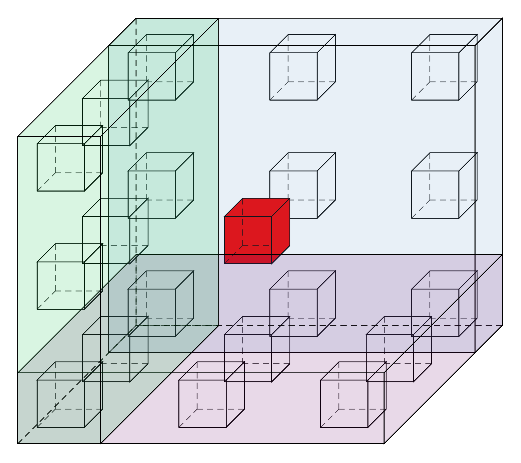
\includegraphics[width=5cm,keepaspectratio]{images/spatial_localization.eps}
            \caption{Intravoxel localization}
            \label{fig:spatial voxel}
        \end{subfigure} & 
        \begin{subfigure}[c]{0.315\textwidth}
            \centering
            \def\svgwidth{5cm}
            \input{images/B0_inhomogeneity_cube.eps_tex}
            \caption{Intravoxel spatial distribution of $B_0$ with minor distortions}
            \label{fig:spatial B0}
        \end{subfigure} &
        \begin{subfigure}[c]{0.315\textwidth}
            \centering
            \def\svgwidth{5cm}
            \input{images/B0_inhomogeneity_cube_severe_distortion.eps_tex}
            \caption{Spatial distribution of $B_0$ with major distortions}
            \label{fig:spatial B0 severe}
        \end{subfigure}
    \end{tabular}
    \caption{Voxels are often treated as singularities, meaning the entire volume is considered to be single point like the red box in the center. Accounting for these intravoxel distributions leads to more accurate and more realistic simulations. \ref{fig:spatial voxel} highlights the spatial nature of voxels while \ref{fig:spatial B0} and \ref{fig:spatial B0 severe} show different levels of intravoxel $B_0$ inhomogeneity.}
    \label{fig:intravoxel localization}
\end{figure}
